
% Bug: automatically loads natbib with name options, cannot be
% overridden, `Elsevier LaTeX' style produces error messages

\documentclass[review]{elsarticle}
%\documentclass{elsarticle}

\usepackage{hyperref}
\usepackage{lineno,hyperref} \modulolinenumbers[5]
\usepackage{graphicx}
\usepackage{mathtools}

\journal{Transportation Research Part C}

%%%%%%%%%%%%%%%%%%%%%%%
%% Elsevier bibliography styles
%%%%%%%%%%%%%%%%%%%%%%%
%% To change the style, put a % in front of the second line of the current style and
%% remove the % from the second line of the style you would like to use.
%%%%%%%%%%%%%%%%%%%%%%%

%% Numbered
\bibliographystyle{model1-num-names}

%% Numbered without titles
%\bibliographystyle{model1a-num-names}
 
%% Harvard
%\bibliographystyle{model2-names.bst}\biboptions{authoryear}

%% Vancouver numbered
%\usepackage{numcompress}\bibliographystyle{model3-num-names}

%% Vancouver name/year
%\usepackage{numcompress}\bibliographystyle{model4-names}\biboptions{authoryear}

%% APA style
%\bibliographystyle{model5-names}\biboptions{authoryear}

%% AMA style
%\usepackage{numcompress}\bibliographystyle{model6-num-names}

%% `Elsevier LaTeX' style
% \bibliographystyle{elsarticle-num}
%%%%%%%%%%%%%%%%%%%%%%%

\begin{document}

\begin{frontmatter}

\title{Formulation and validation of a car-following model based on
  reinforcement learning}

%% Group authors per affiliation:
%\author{Fabian Hart\fnref{myfootnote}}
%\address{TU Dresden}
%\fntext[myfootnote]{Comment.}

%% or include affiliations in footnotes:
\author[firstAddress]{Fabian Hart}
\author[firstAddress,secondAddress]{Ostap Okhrin}
\author[firstAddress,secondAddress]{Martin Treiber\corref{corrAuthor}}
\cortext[corrAuthor]{Corresponding author}
\ead{Martin.treiber@tu-dresden.de}
\ead[url]{www.mtreiber.de}

\address[firstAddress]{TU Dresden}
\address[secondAddress]{Possible second address}




\begin{abstract}
To be written at the end
\end{abstract}

\begin{keyword}
reinforcement learning \sep car-following model \sep stochastic
processes \sep string stability \sep validation \sep trajectory data 
\end{keyword}

\end{frontmatter}

%\linenumbers

\section{Introduction}

[problem statement]

[references for state-of-the art]
references RL: \cite{farazi2020deep,qu2020jointly}
references classical, ACC, stochastic CF model: 
\cite{Opus,TreiberKesting-Book,Treiber2018stochIDM_TRB}
%references full2D: \cite{Kanagaraj2018self}
references AR(1), e.g. \cite{HonerkampEngl}


[central statement] To our knowledge, no neuronal-network car-following model has been proposed that considers such high safety and comfort standards, that considers the transition between free driving and car following and that shows string-stability.
In this contribution, we propose a novel reinforcement learning (RL)
car-following model that is trained on leading-vehicle trajectories
generated by an AR-1 process with parameters reflecting the kinematics of real
leaders. We validate the trained model on experimental and
naturalistic trajectory data, and on artifical speed profiles
bringing the model to its limits. In all cases, the model proved to be accident
free and  string stable. Unlike other variants of RL car-following models our approach considers a wider range of possible accelerations in a way, that full-braking scenarios can be successfully mastered. Also, unlike
other variants of AI models such as LSTM models trained on realistic data, the proposed model is
not completely blackbox since the reinforcement learning reward
function reflects driving style attributes such as desired time gap and
speed, maximum acceleration, and comfortable deceleration. 

[short textual enumeration of the sections to come]

\section{Model specification}
The Follower Vehicle is designed to be controlled by a Reinforcement Learning (RL) agent. By interaction with an environment, the RL agent optimizes a sequential decision making problem. At each time step $t$ the agent observes an environment state $s_t$ , and based on that state selects an action $a_t$. After conducting action $a_t$, the RL agent receives a reward $r(a_t,s_t)$. The agent aims to learn an optimal state-action mapping policy $\pi$ that maximizes the expected accumulated discounted reward $r_{t}=\sum_{k=0}^{\infty} \gamma^{k} r_{t+k}$, with $\gamma = (0,1]$ describing the discount factor. The crucial elements
of the Reinforcement Learning based control strategy are described
in detail as follows:

\subsection{Action space}
\label{actionSpace}
In this study, the acceleration of the Follower Vehicle is considered as the action of the RL agent. To maintain  comfortable driving and to allow full-brake in safety-critical situations the acceleration is a continuous variable between $a_{min} = -9m/s^2$ and $a_{max} = 2m/s^2$.


\subsection{State space}
The state space defines the observations, the Follower Vehicle can receive from the environment. To compute an optimal acceleration, the Follower Vehicle observes its own acceleration $a$, its own velocity $v$, the difference velocity $\Delta v$ and the spatial distance to the Leading Vehicle $s$. These observations were normalized to the range $[-1,1]$.


\subsection{Reward Function}
The goal of the RL strategy is to reduce the crash risk, while maintaining comfortable driving in non-safety-critical situations. The Reward function is based on a set of parameters, that can be adjusted to realize different driver styles. $v_{des}$ is the desired velocity, that should not be exceeded. $a_{min}$ and $a_{max}$ are the minimum and maximum possible accelerations, as described in Section \ref{actionSpace}. All parameters are described in Table \ref{tab:agentParameters}.

\begin{table}
\caption{RL agent parameters} 
\label{tab:agentParameters} 
\begin{center}
\begin{tabular}{ p{0.12\textwidth} p{0.65\textwidth} p{0.1\textwidth}}
	Parameter & Description & Value \\ \hline
	$a_{min}$ & Minimum acceleration & $-9m/s^2$ \\  
	$a_{max}$ & Maximum acceleration & $2m/s^2$ \\  
	$b_{comf}$ & Comfortable deceleration & $2m/s^2$ \\  
	$v_{des}$ & Desired velocity & $16.6 m/s$ \\  		
	$T_{gap}$ & Desired time gap to Leader & $1.5s$ \\
	$s_{min}$ & Desired minimum distance to Leader & $2m$ \\
	$T_{var}$ & Time gap to describe the variance of the normal probability function (see Figure xy) & $0.7s$ \\
	$T_{lim}$ & Upper time gap limit for zero reward (see Figure xy) & $15s$ 
\end{tabular}
\end{center}
\end{table}


The reward function consists of four parts, described as follows:


\begin{equation}
r_1  = 
\begin{cases}
\frac{normpdf(s,  s_{opt},  s_{var})}{normpdf( s_{opt},  s_{opt},  s_{var})},& \text{if } s < s^*\\
\frac{normpdf(s^*,  s_{opt},  s_{var})}{normpdf( s_{opt},  s_{opt},  s_{var})} (1-\frac{s-s^*}{s_{lim} - s^*})              & \text{otherwise}
\end{cases}
\end{equation}



with
\begin{equation}
s_{opt} = vT_{gap} + s_{min}
\end{equation}
\begin{equation}
s_{var} = vT_{var} + 0.5s_{min}
\end{equation}
\begin{equation}
s_{lim} = vT_{lim} + 2s_{min}
\end{equation}
The first part of the reward function aims to maintain a reasonable distance to the Leader Vehicle.
Normpdf(x,$\mu$,$\sigma^2$) describes a normal probability density function. Figure \ref{fig:RewardFunc1} illustrates the reward function for $r_1$, containing the parameter $s^*$, $s_{lim}$ and $s_{opt}$. The reward function is designed in a way, that for high velocities of the Follower Vehicle the time gap between Follower and Leader Vehicle tends to $T_{gap}$, while for low velocities the distance between both tends to $s_{min}$. Different values of $T_{opt}$ result in different driving styles in a way, that for higher values of $T_{opt}$ the Follower drives up closer, resulting in a more aggressive driving style. The results for different values of $T_{opt}$ can be found in Section xy. Different functions for $ s > s^*$ has been applied, but the best results regarding a smooth and comfortable approaching of the Follower Vehicle has been reached with a linear function. Also, a high value of $T_{lim}$ results in an early deceleration and comfortable approaching. 

\begin{figure}
	\centering
	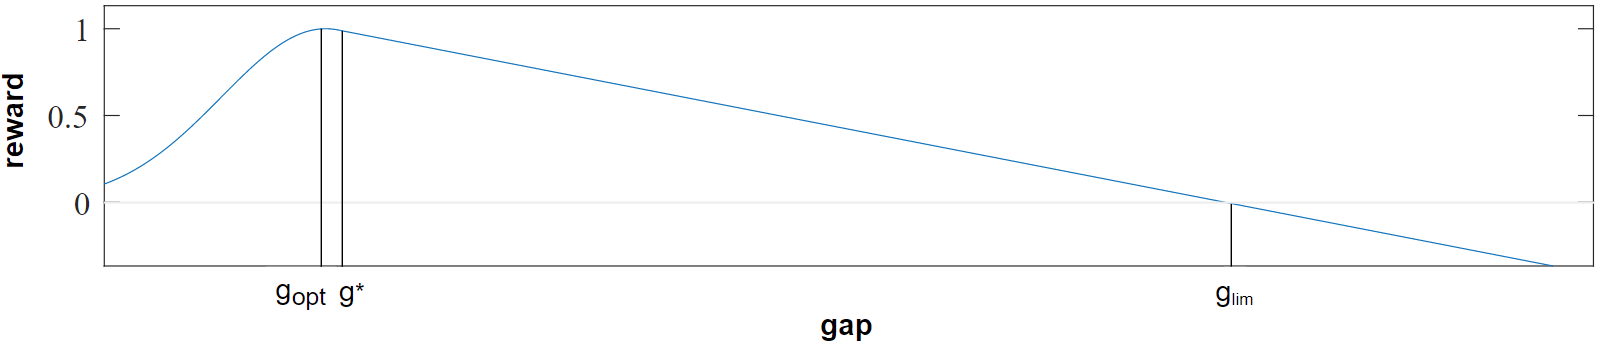
\includegraphics[width=12cm]{images/RewardFunc1}
	\caption{Reward function part 1 maximizes the reward for car following with time gap $T_{gap}$.}
	\label{fig:RewardFunc1}
\end{figure}


\begin{equation}
r_2 = 
\begin{cases}
\tanh\left(\frac{b_{kin}-b_{comf}}{a_{min}}\right),& \text{if } b_{kin}>b_{comf}\\
0,              & \text{otherwise}
\end{cases}
\end{equation}

with
\begin{equation}
b_{kin} = \frac{\Delta v^2}{s}
\end{equation}
The second part of the reward function addresses the vehicle behavior in safety-critical situations.
For a deceleration with the delay $b_{kin}$ the braking distance is equal to the current distance $s$. Thus, the kinematic deceleration represents the minimum deceleration necessary to avoid a collision. A situation is considered as "safety-critical", if the kinematic deceleration $b_{kin}$ is greater than the comfortable deceleration $b_{comf}$. Thus, just in safety-critical situations the RL agent is getting penalized, illustrated in figure xy.

\begin{equation}
r_3 = -\left(\dfrac{da}{dt}\right)^2
\end{equation}

The third part of the reward function aims to reduce the jerk in order to achieve a comfortable driving. 

\begin{equation}
r_4 =  
\begin{cases} 
 -min\left(1,\left( v - v_{des}\right)^2\right), & \text{if } v>v_{des}\\
0, & \text{otherwise}
\end{cases}             
\end{equation}

The fourth part of the reward function penalizes the RL agent, if the current velocity is above the desired velocity $v_{des}$. 

\begin{equation}
r = 0.6r_1 + 1.1r_2 + 0.001 r_3 + r_4
\end{equation}

The weights of each reward part has been found experimentally and can further be optimized in future studies.

\subsection{RL algorithm}
In various similar control problems, the Deep Deterministic Policy Gradient (DDPG) Algorithm has been used and proven to perform well on tasks with a continuous action and state space (see xyz). In order to reduce the variance of policy gradients and increase learning speed, DDPG is an actor-critic method. The actor determines the action, while the critic judges about the quality of the action and how the policy should be adjusted. ([-> original paper DDPG])Both, actor and critic, are implemented as neural networks. In this study, both networks are feed-forward neural networks with two layers of hidden neurons and 32 neurons each hidden layer. All DDPG parameters are presented in Table \ref{tab:DDPGparameters}

\begin{table}
	\caption{DDPG parameter values} 
	\label{tab:DDPGparameters} 
	\begin{center}
		\begin{tabular}{ p{0.4\textwidth} p{0.2\textwidth} }
			Parameter & Value \\ \hline
			Learning rate & 0.001 \\ 
			Reward discount factor & 0.95 \\ 
			Experience buffer length & 100000 \\ 
			Mini batch size & 32 \\ 			
			Gaussian noise mean & 0.15 \\ 
			Gaussian noise variance & 0.2 \\ 
			Gaussian noise variance decay  & 1e-5 \\ 
			Number of hidden layers & 2\\
			Neurons per hidden layer & 32\\
			

		\end{tabular}
	\end{center}
\end{table}


\subsection{Reward function}

learning input (leader speed time series)

[also relate parameters to driving style attributes such as desired
speed, accelerations, decelerations, desired time gap, minimum gap]


\section{Model training}

\subsection{Synthetic trajectories}

(truncated) AR(1) process of the leading speed

parameters and statistical properties (expectation, variance, auto-correlation
function, typical accelerations

figure of realisation

\begin{figure}
	\centering
	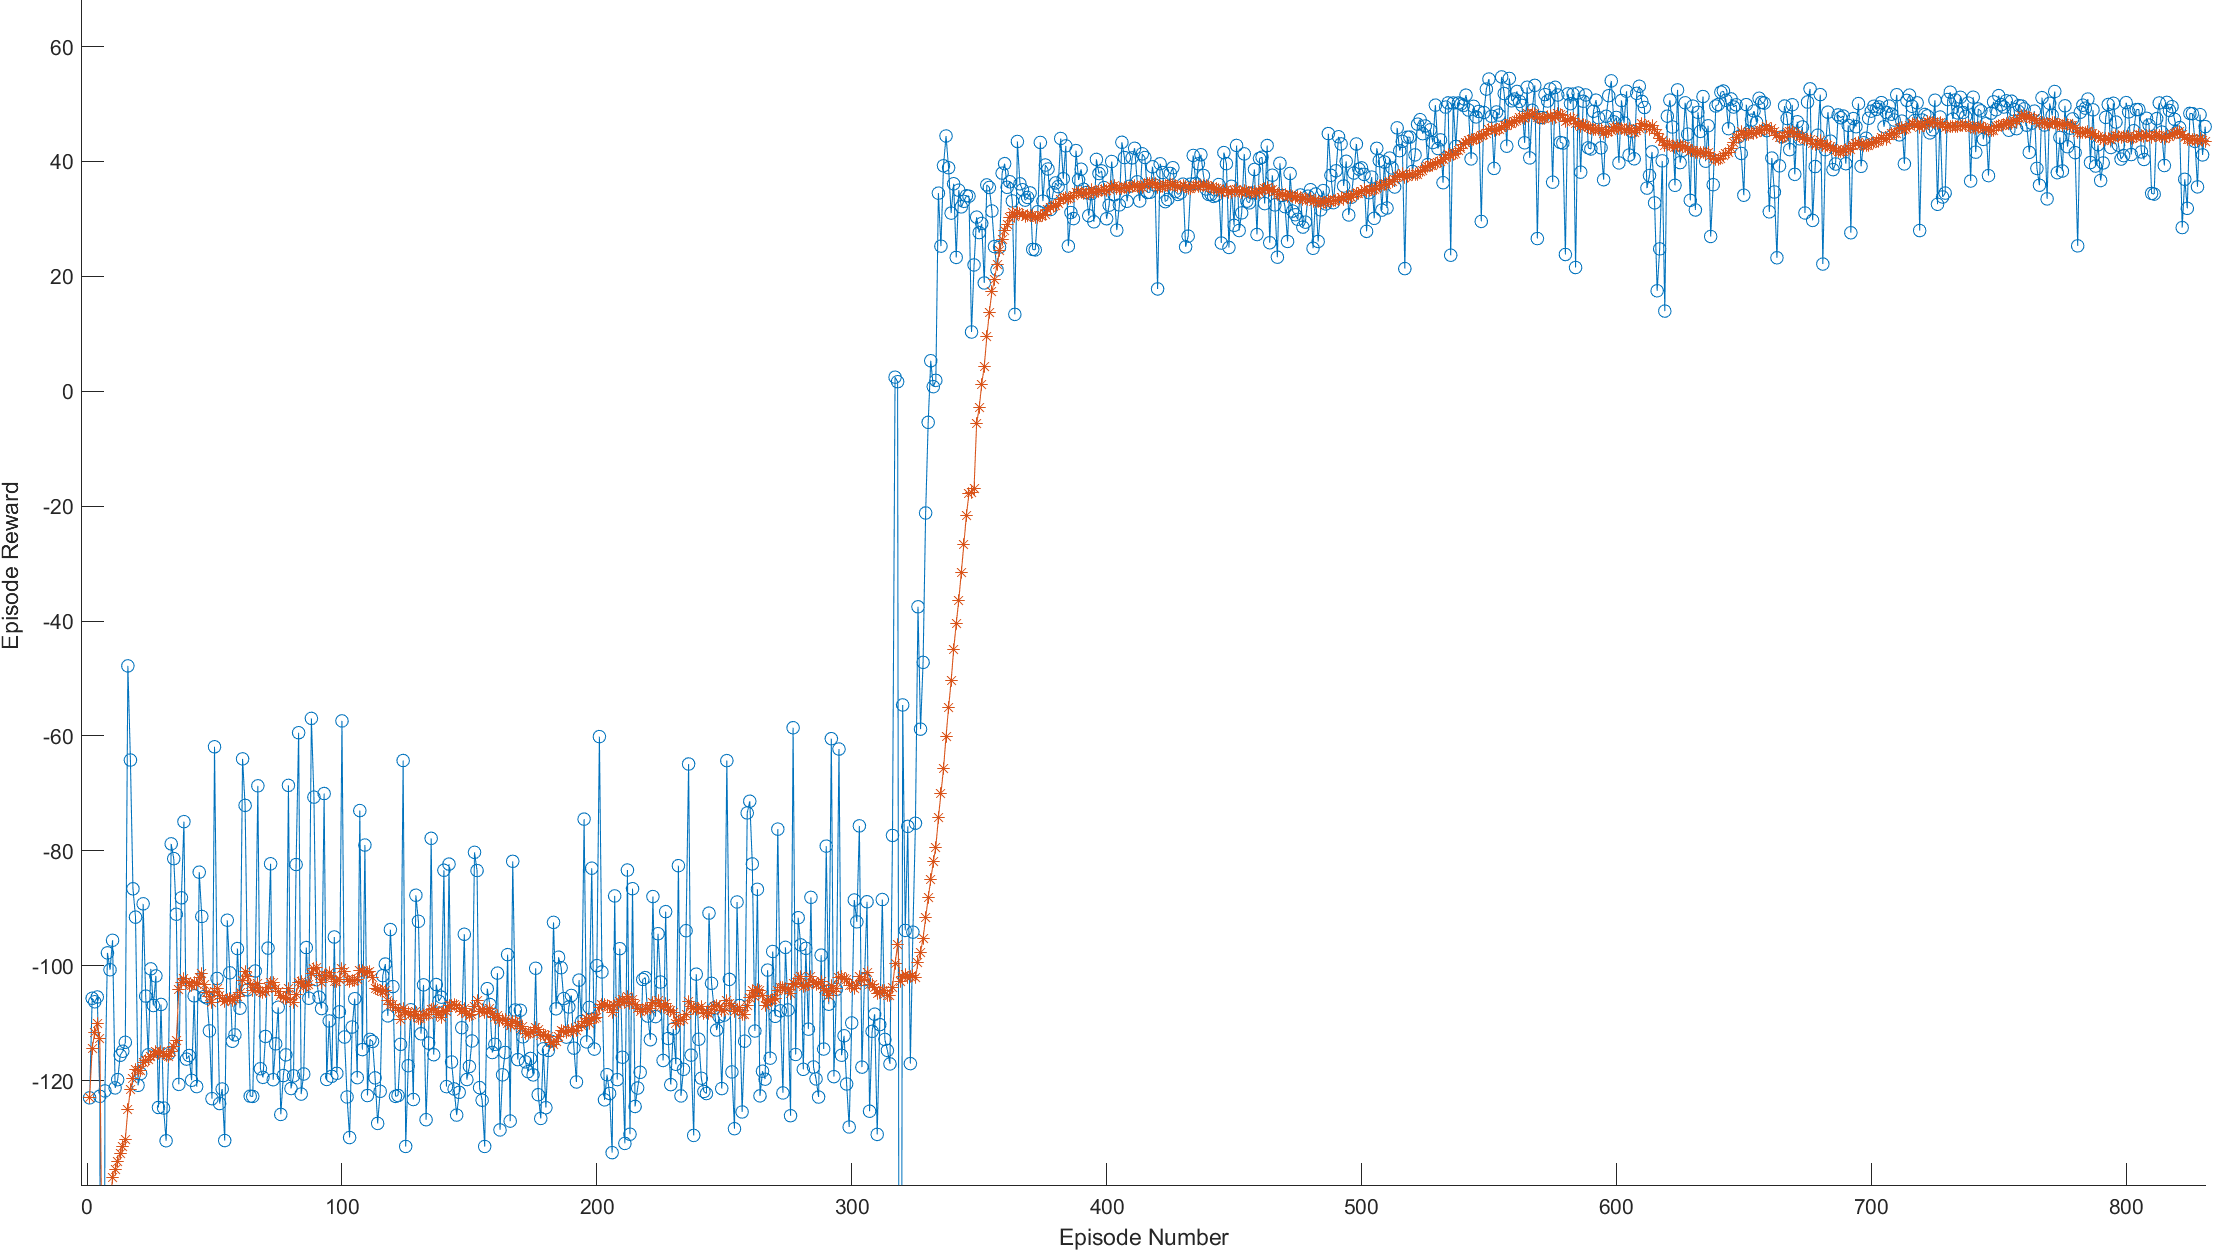
\includegraphics[width=12cm]{images/Training}
	\caption{Training process}
	\label{fig:training}
\end{figure}

\subsection{Evaluation of the reward function}

[implementation of the AR(1) process, numerical integration of the
  model output (acceleration?): numerical scheme, update time etc]

\subsection{The reinforcement learning process}

[things to look out for]

[typical figure of increasing reward over \#steps, then saturation]

[number of steps, computing time]

[figure of following trajectory instance at the beginning and after
  saturation of the 
  learning process]


\section{Validation}

The goal is not to minimize some error measure as in usual
calibration/validation but to check if the driving style is safe,
effecetive, and comfortable. Reference for this is the reward function

\subsection{string stability}

many trained RL vehicles behind the AR(1) realisation

\begin{figure}
	\centering
	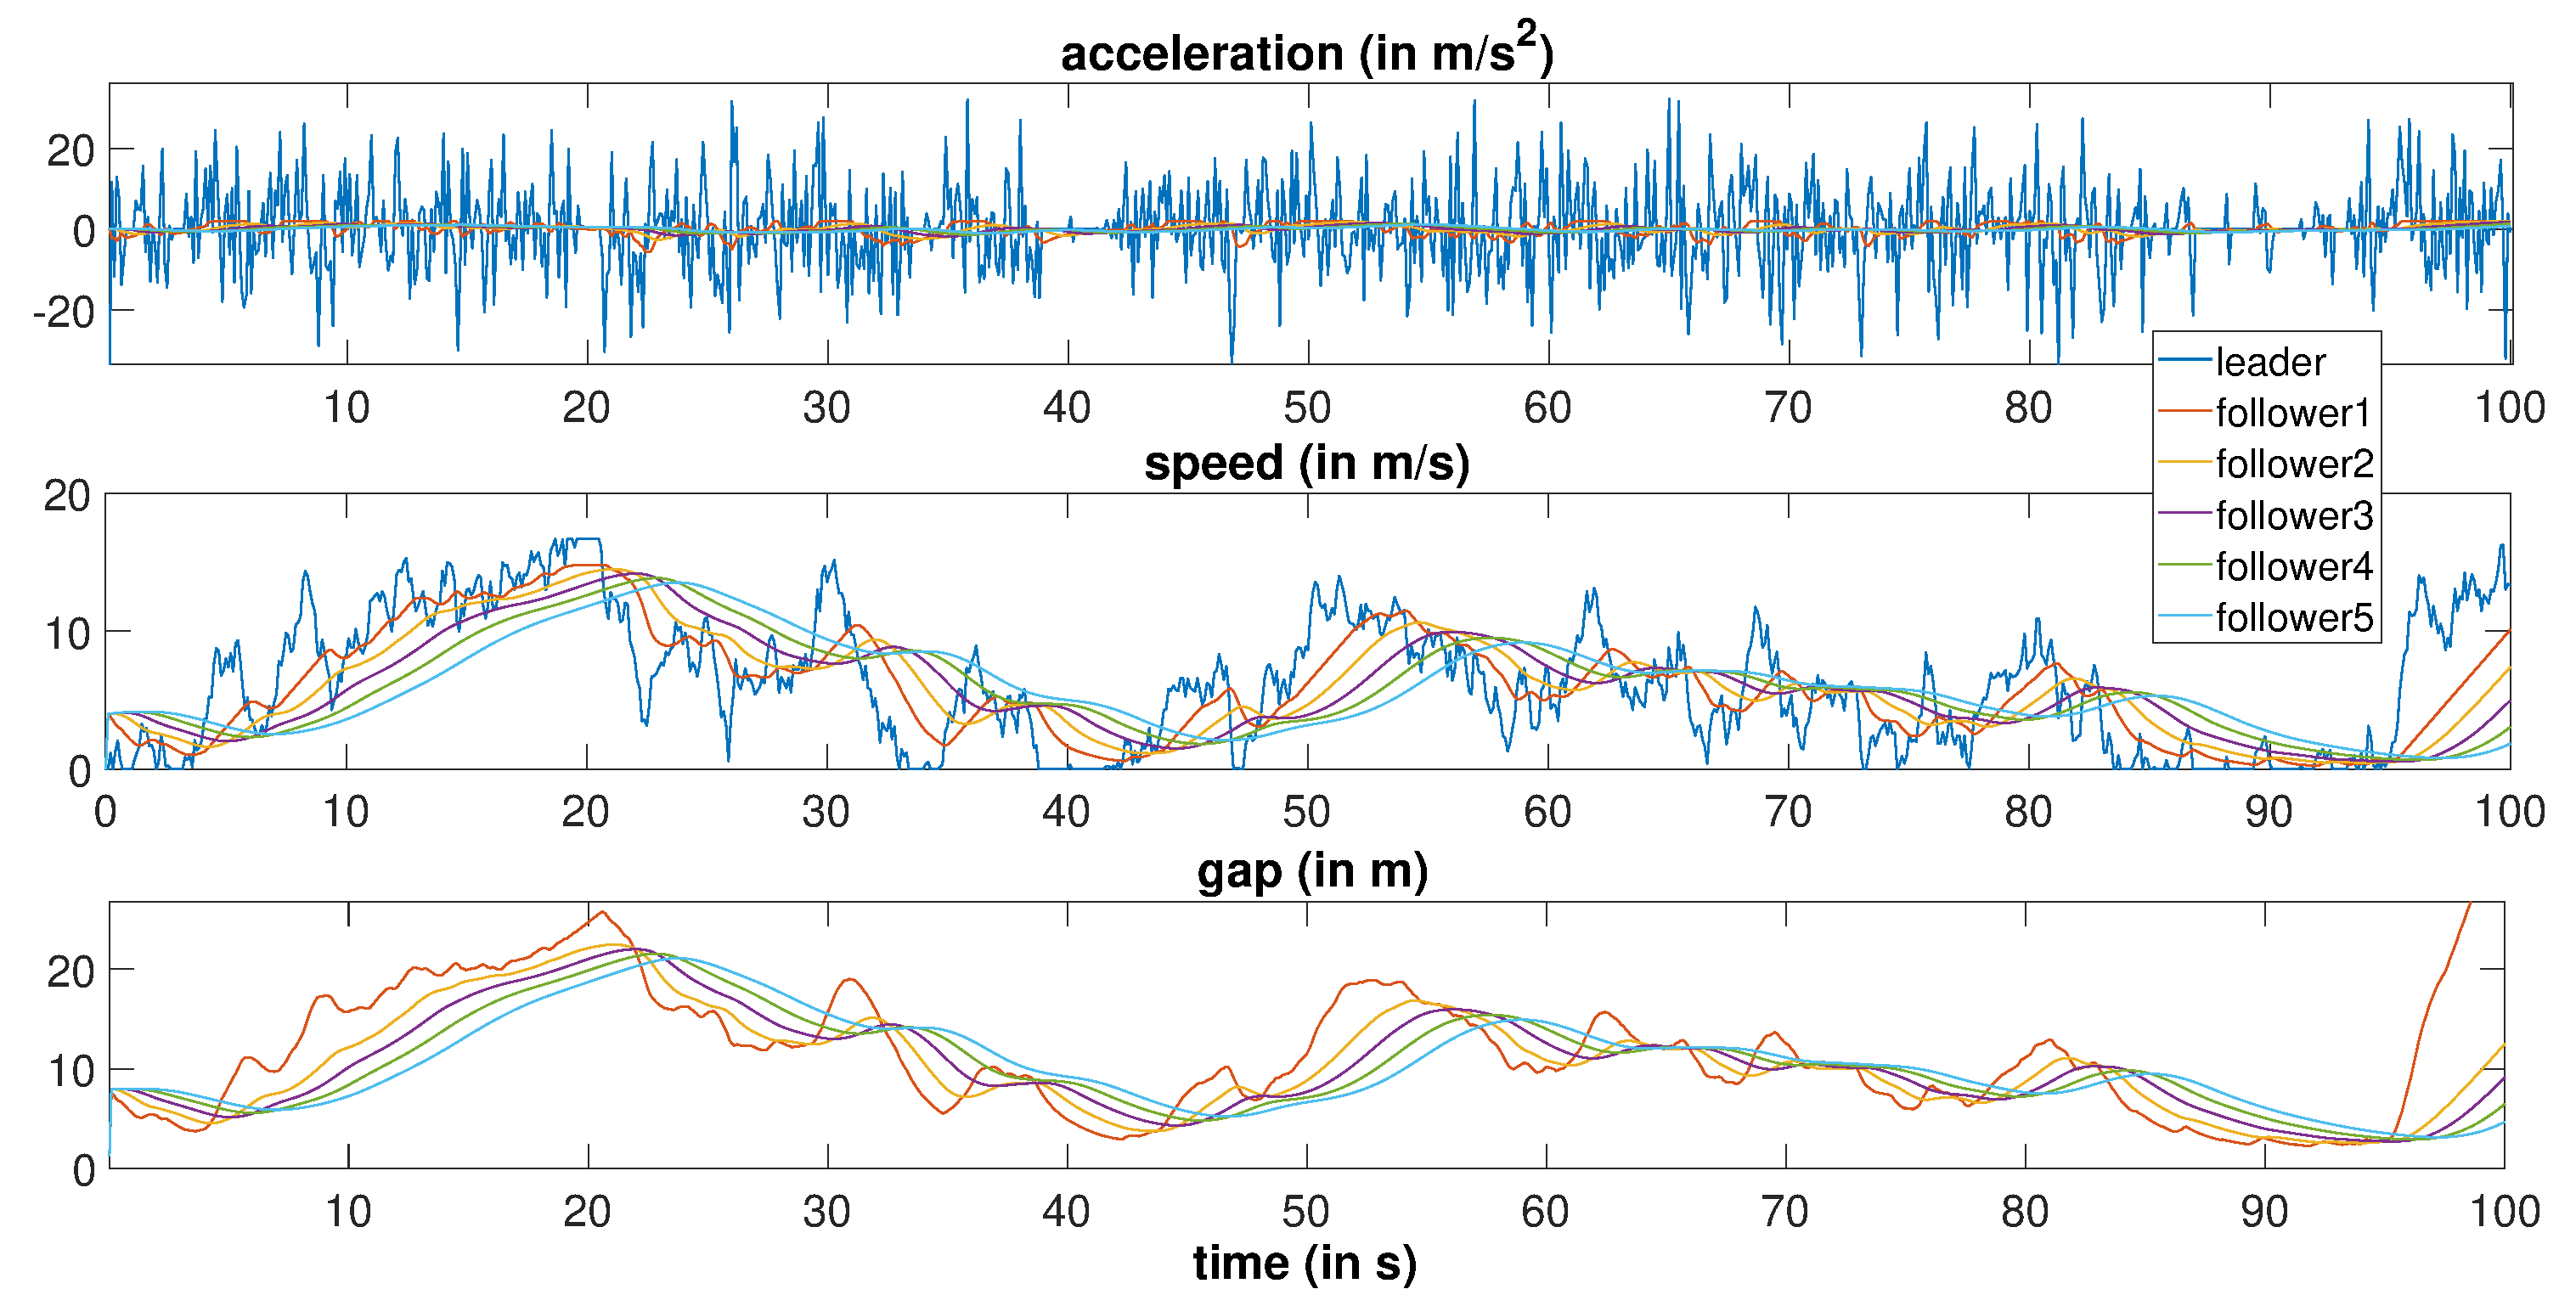
\includegraphics[width=12cm]{images/AR1Kolonne}
	\caption{}
	\label{fig:AR1Kolonne}
\end{figure}

\subsection{Response to an external leading vehicle speed profile}

[decribe profile with episodes of free driving, dynamic approaching,
  car-following, stopping, accelerating, and traffic waves]

\begin{figure}
	\centering
	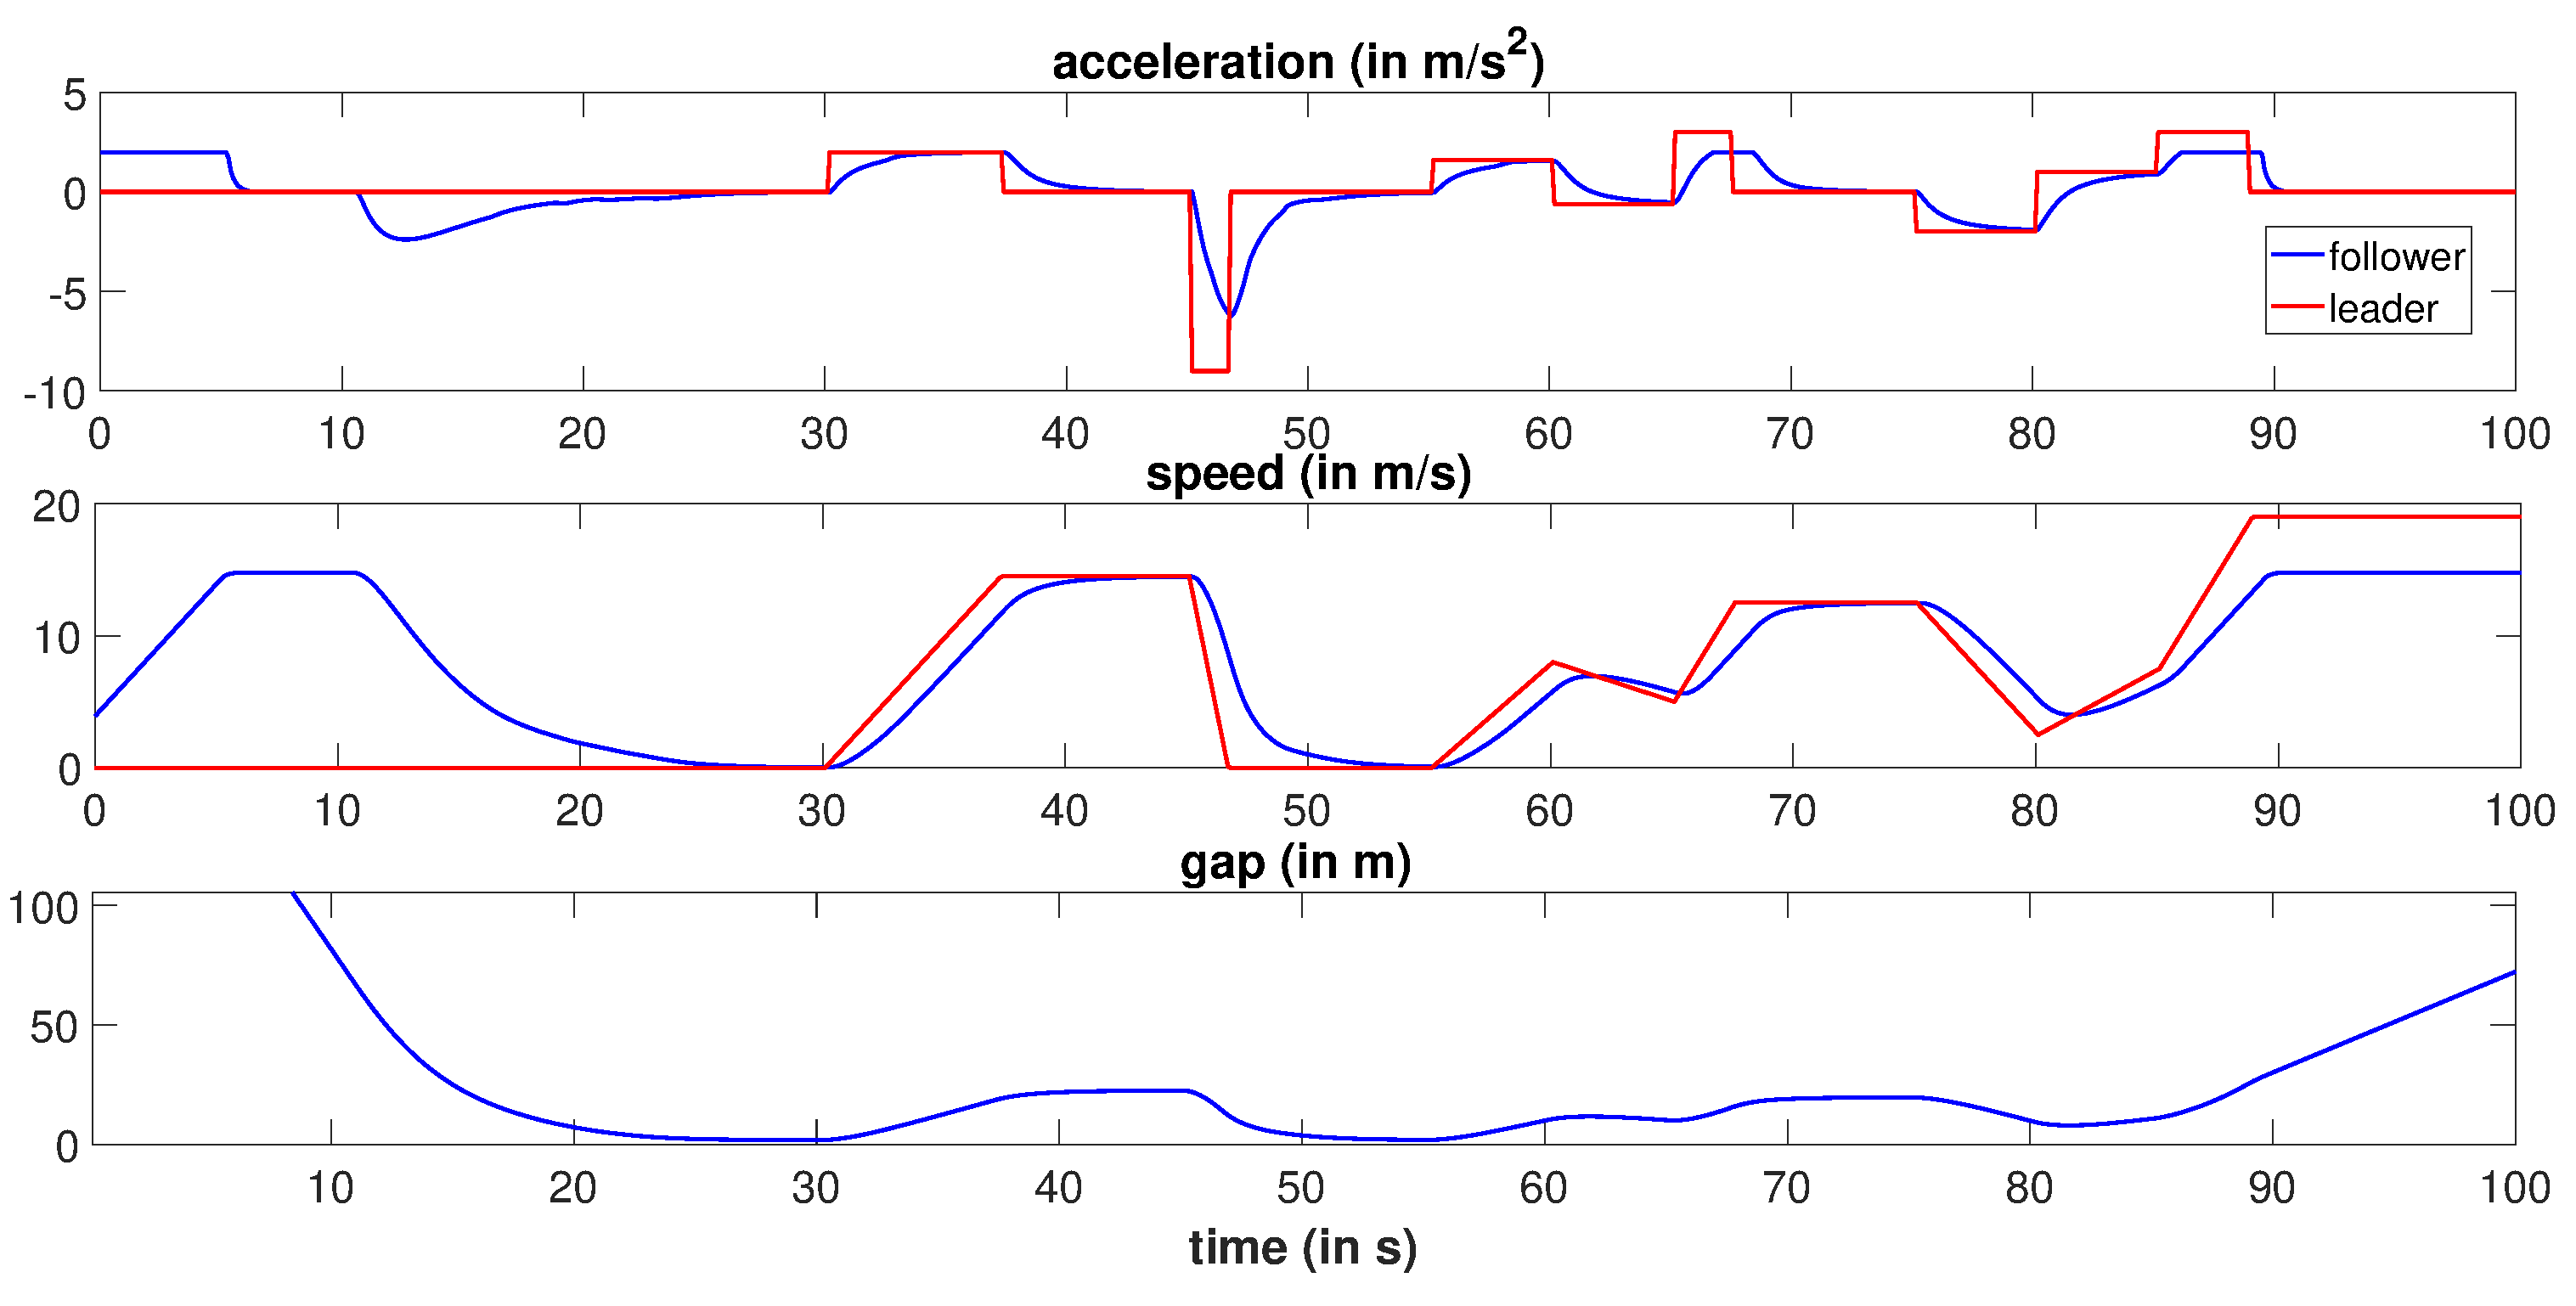
\includegraphics[width=12cm]{images/manipulatedLeader.eps}
	\caption{}
	\label{fig:manipulatedLeader}
\end{figure}

[discussion: free: desired speed; following: desired time gap; dynamic
  situations: accelerations, desired and maximum  decelerations, jerk;
comfort: maximum accelerations, decelerations, jerk;
  safety: no crashs, minimum TTC; stability: string stable]


\subsection{Response to experimental leaders}

[describing the Napoli data]

[figure with several followers]

\begin{figure}
	\centering
	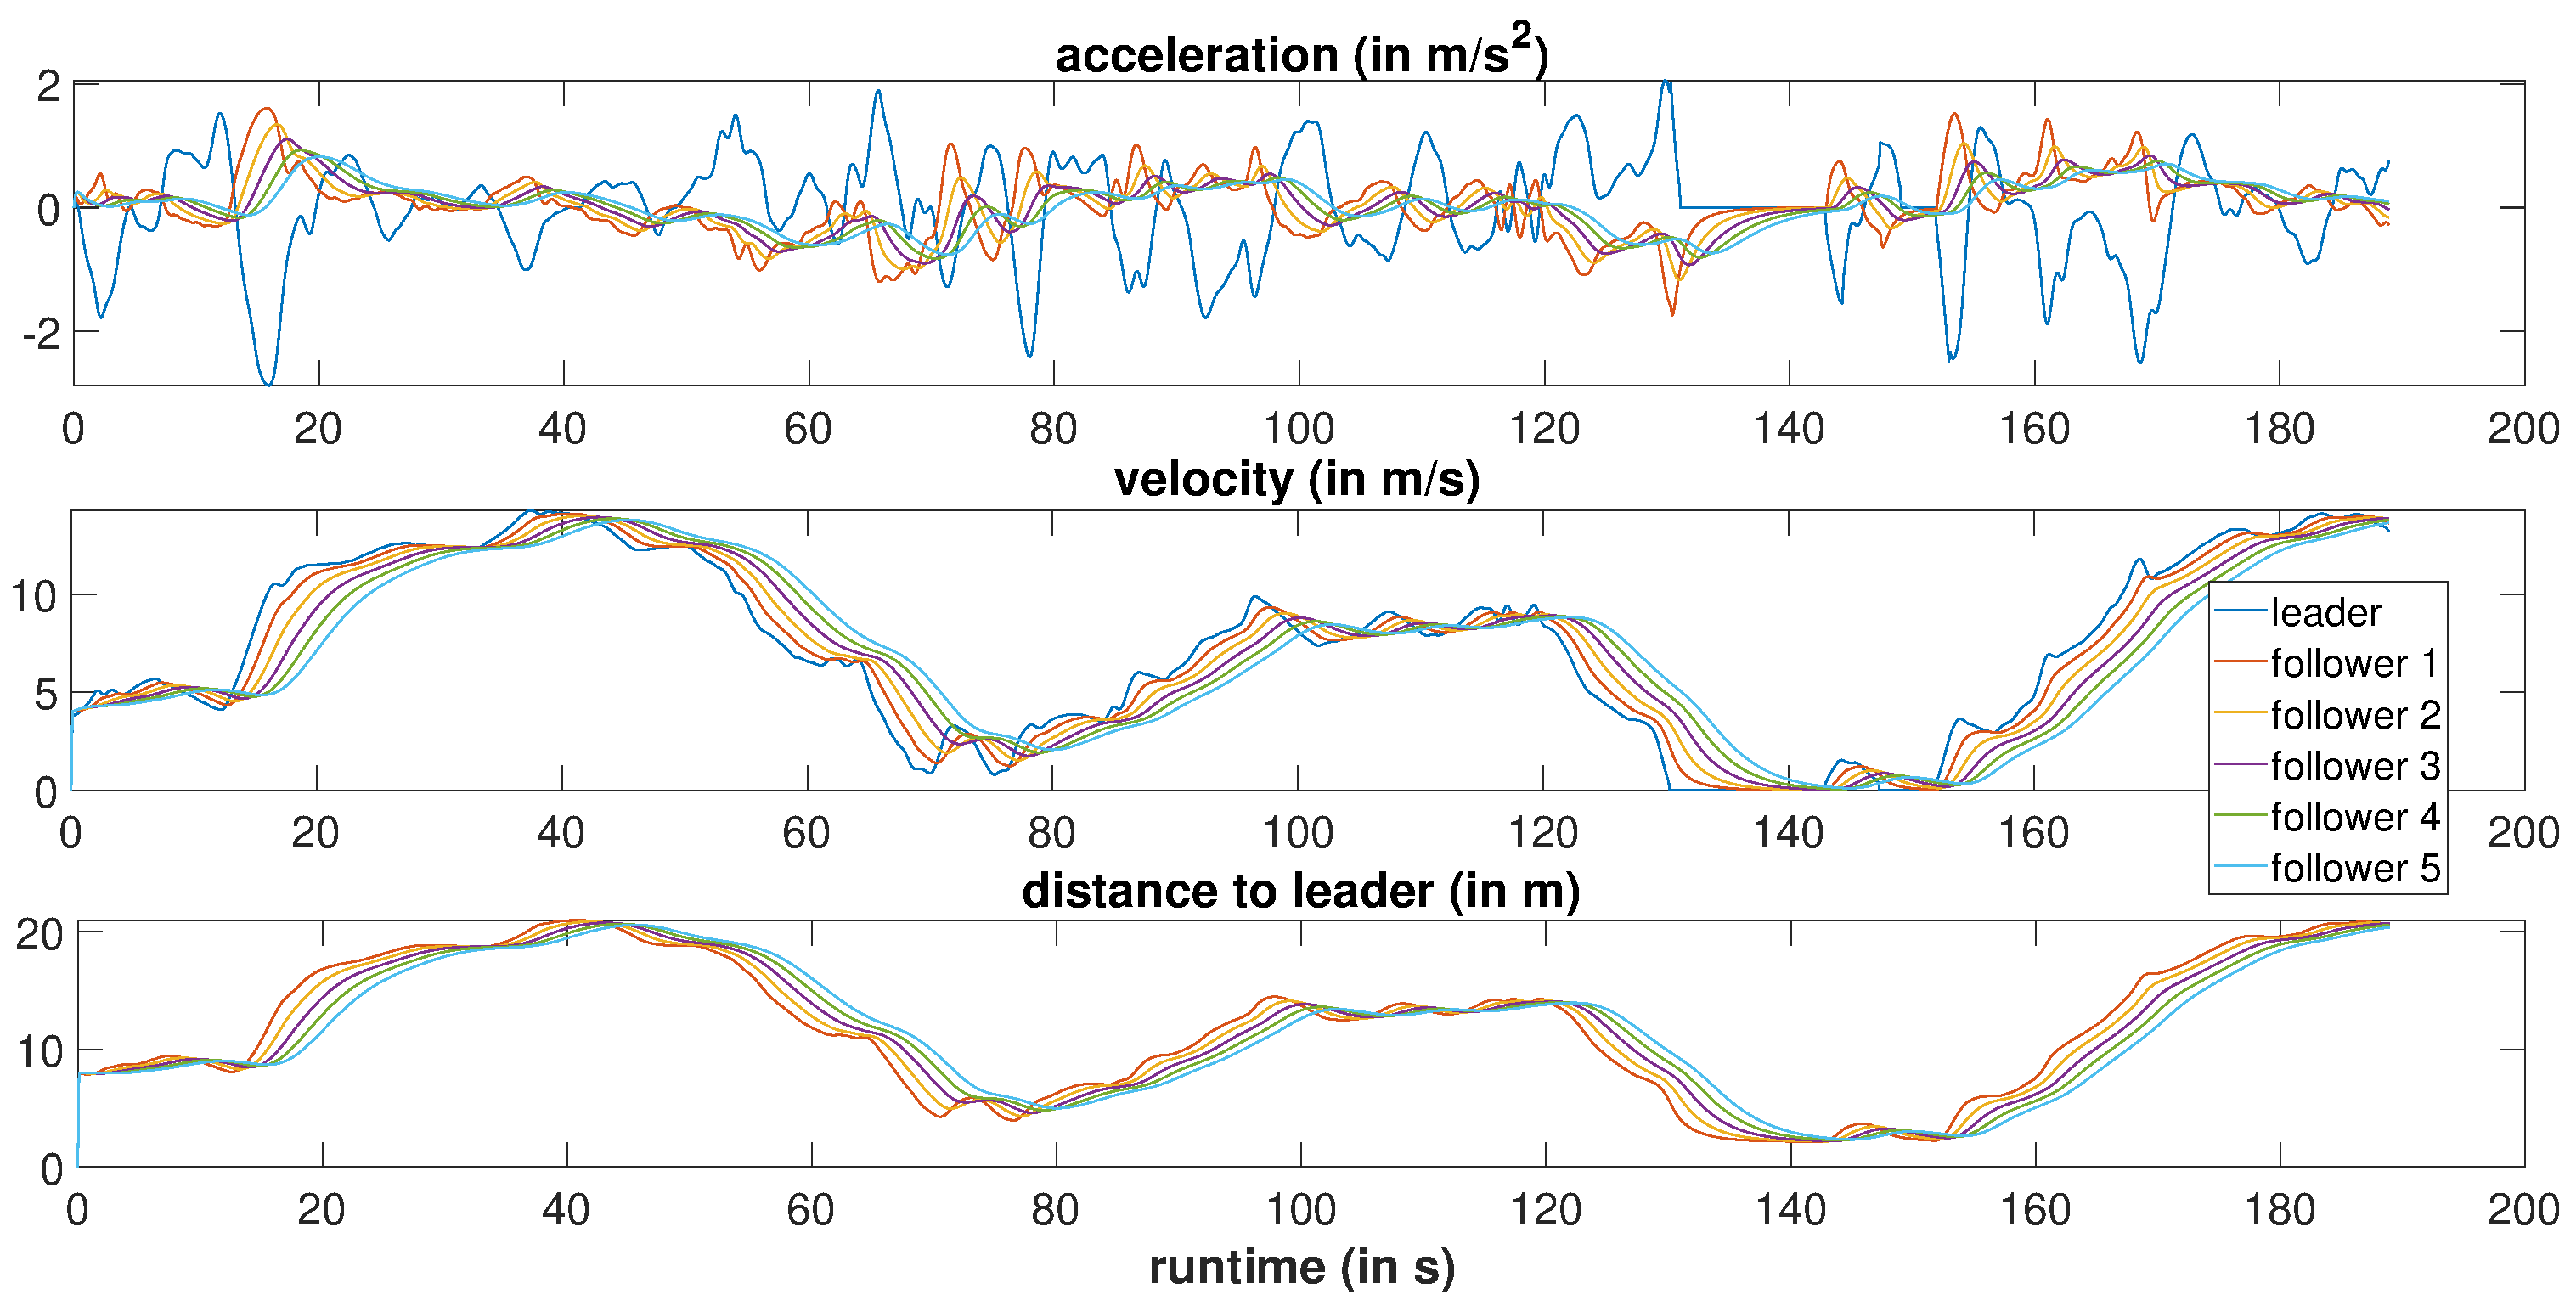
\includegraphics[width=12cm]{images/PunzoKolonne}
	\caption{}
	\label{fig:PunzoKolonne}
\end{figure}

[cross comparison with IDM calibrated to this set]
2x2 table; rows: RL model and IDM;
columns: reward function and calibration GoF (goodness-of-fit) function

\subsection{Repsonse of different driver characteristics to experimental leaders }

\begin{figure}
	\centering
	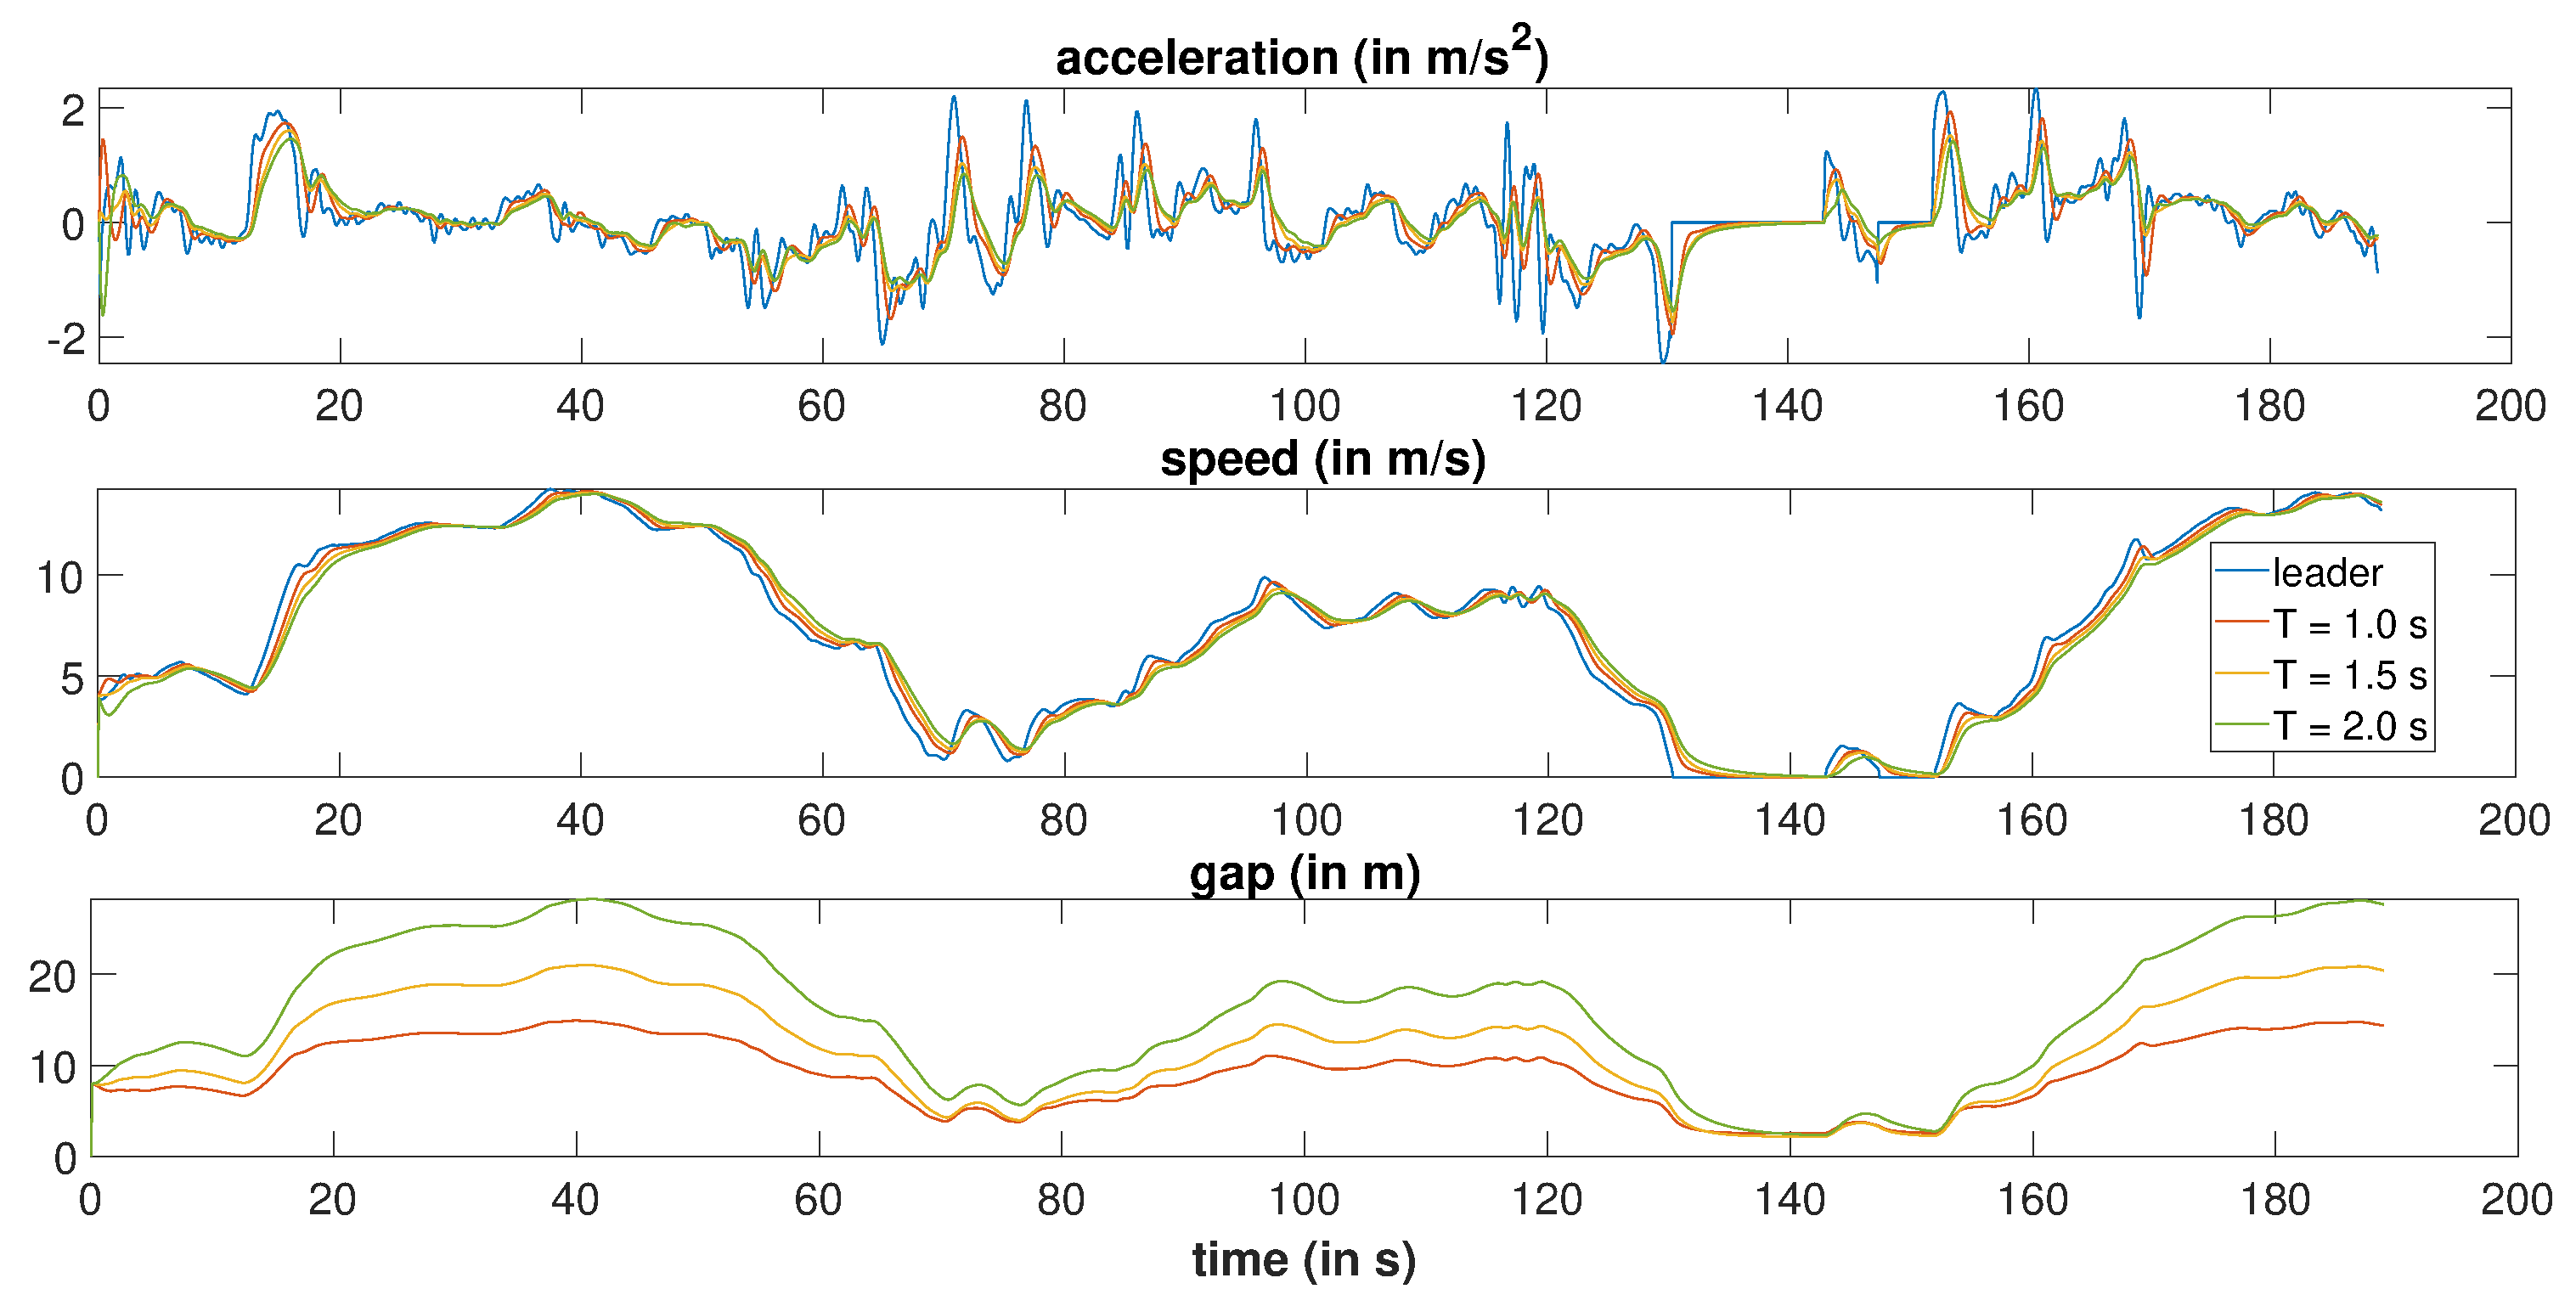
\includegraphics[width=12cm]{images/differentT}
	\caption{}
	\label{fig:differentT}
\end{figure}


\subsection{Simulation of collective phenomena}

[open system with speed-limit or on-ramp bottleneck (simplest vehicle
  dropping), increase inflow until breakdown to determine capacity,
  stability: no traffic waves, just congested traffic, maximum
  deceleration at the upstream jam front, propagation velocities]


\section{Conclusion/Discussion}

\section*{References}

\bibliography{RL_vehicles_references}

\end{document}
